\chapter{Robocup2d足球的入门}
\section{2D仿真足球的简介}
1997年是人工智能领域发展中的重要一年,该年5月IBM的机器人“深蓝”击败了人类国际象棋冠军,揭开了人工智能领域的崭新一页。同年首届Robocup比赛及会议在日本名古屋举行,迈出了实现机器人足球击败人类足球世界冠军这一梦想的第一步。

Robocup(Robot World Cup),即机器人世界杯足球赛,它涉及人工智能、机器人学、通讯、传感等诸多领域的前沿研究和技术集成。是在动态不确定环境下对人工智能的考验,是培养信息、自动化领域科技人才的重要手段。而2D仿真足球就是机器人足球世界杯仿真组比赛中的一个类别,是在二维空间角度对足球赛的一种仿真。由于不需要较多的资金投入,仿真组的比赛是目前参赛队伍最多的比赛。



\section{2D仿真足球的仿真过程}
Robocup 2d仿真足球比赛的仿真平台软件rcsoccersim(RoboCup Soccer Simulator),该平台包括一个简单的仿真机器人例程rcssclient,仿真比赛监视程序rcssmonitor,仿真比赛重播程序rcssslogplayer和最主要的仿真比赛服务器程序rcssserver。

比赛时,各参赛队将自己编写好的仿真足球程序加载到仿真平台上去,让其在rcsoccersim提供的虚拟场地自主的进行比赛。比赛采用Client/Server模式,简称C/S结构,每个Client模块只允许控制一名机器人,Client之间不允许直接进行通信,只能通过Server服务器才能进行通信,Server服务器实际上控制着整个比赛。

Server与Client之间的通信都是通过UDP/IP协议来实现的,所以Client的开发和运行环境只需支持UDP/IP协议即可。Server服务器包括两个程序:Soccer Server和Soccer Monitor。其中,Monitor是比赛监视器,显示虚拟场地;Server可以与多个Monitor相连在多个显示器上同时显示比赛情况。客户端程序分为以下四种类型,其中球员智能体,智能体教练,训练师智能体被统称为足球智能体。
\begin{figure}[H]
	\centering 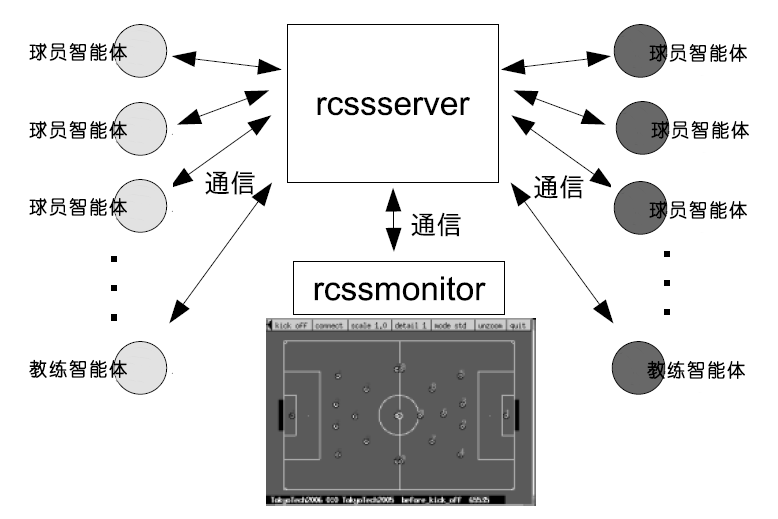
\includegraphics[width=0.65\textwidth]{server.png}
	\caption{2D仿真模拟的结构}
\end{figure}

\begin{itemize}
	\item \textbf{球员智能体}
	
	可以控制场上的球员。不但能得到成段的信息,只有得到部分的、包含噪声的信息。
	\item \textbf{教练智能体}
	
	能够获得关于对象的完整的位置信息。能给予球队意见,但不能直接控制球员。它在比赛过程中使用。
	\item \textbf{训练器智能体}
	
	它除了具有教练的能力,还可以控制同一场比赛中的裁判。它不能在比赛过程中使用。所以也被称为离线教练。
\end{itemize}
\section{2D仿真足球的特点}

通过上面的介绍,可以看到,作为一个试验平台,这套仿真比赛平台提供了一个很好的
全分布的、包括合作与对抗的多主体实时环境,非常有挑战性。其具体特点如下:
\begin{itemize}
	\item \textbf{分布式多主体团队合作和对抗}  所有客户端程序分别控制场上的一名球员或教练,
	自主决策,分布运行,队友之间有合作,对手之间有对抗
	\item \textbf{动态、实时、不确定环境}  在服务器端,整个系统按照100 毫秒的周期运转,所有
	球员都必须按照这个周期运行,意味着球员的所有决策都必须实时完成,由于多主体
	的存在,环境在动态的转变,无法预知(这也被称为“不透明转换”[Stone 1998])。
	\item \textbf{感知和行为异步}  由于比赛时间以周期为单位离散,感知和行为就无法同步,所以
	光靠传统人工智能方法使用感知来激发行动是远远不够的
	\item \textbf{球员能力受限}  场上所有球员能力都是参照真实球员有所限制的,如体力、加速度、
	最大速度、惯性等
	\item \textbf{视觉受限}  每个球员的视觉都是局部的,收到球员视角、和视距的限制,也就是说
	球员在任何时刻都只能获得一部分球场上的信息。这就给球员正确分析场上形势,进
	而产生决策带来了困难
	\item \textbf{通讯受限}  球员之间的通讯环境具有单信道、窄带宽等特点,即每队球员公用一条
	信道,每个球员一个周期内只能“听”到队友一条消息,而且信道容量很有限(缺省
	为10 字节)。这样,现有的一些团队合作理论就很难直接应用,因为目前大部分合作
	理论前提都是要求通讯是及时的、完全的
	\item \textbf{多噪声源}  为了真实模拟实际比赛,仿真世界里球员感知和动作都带有噪声,使得
	球员既无法精确地感知世界也不能完全按照它的意图影响世界
	\item \textbf{连接不可靠}  平台网络连接使用UDP/IP,不确保所有信息的正确及时,在网络繁忙
	时一些信息甚至会丢失,这也体现了比赛环境的不确定性,球员程序必须能够适应这
	一环境。
\end{itemize}

\section{基本模型与基本命令}
\subsection{时间模型}
rcssserver是一个离散时间仿真。定期更新其中的状态,对象的位置将仅在该时间更新。这在rcssmonitor中被显示为这个比赛仿真的时间。信息是定期周期更新的,但是,每个智能体的发送和接收消息是与该周期异步完成的。

通常情况下,场内的状态被认为是100毫秒更新一次。因此,理想情况下,rcssmonitor将以每秒10帧更新显示。

\subsection{物理模型}
rcssserver的物理模型与现实世界有很大的不同。例如,地面和物体之间的摩擦系数不考虑,速度衰减率被速度参数所取代。这是因为,它不是现实世界的完全仿真平台,rcssserver被设计为能够流畅运行多智能体仿真环境的仿真平台。



\subsection{球场坐标系}
rcssserver内部的坐标系统使用左手坐标系统. rcssmonitor领域的正确查看方式是,以原点场为中心,向右为X轴正方向,向下是Y轴正方向。它角度的规定也是遵守这样的规则。换句话说,从场中心,右方为0度起算线,左侧方向是180度,向上为-90度,向下为90度。当进行角度计算时,任何时候正方向都是顺时针方向。

如下图所示,该区域的大小是长105米、宽64米。场中心为原点,图形的每个边角的坐标值如图所示。
\begin{figure}[htb]
	\centering 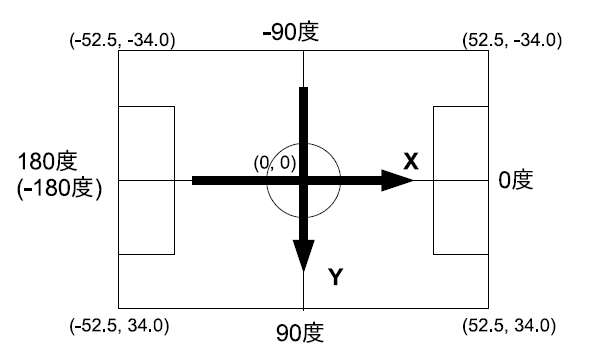
\includegraphics[width=0.65\textwidth]{playground.png}
	\caption{球场坐标}
\end{figure}
\subsubsection{播放系统的坐标}

球员智能体的坐标系统与rcsserver的坐标系统略有不同。在左侧的球队与rcssserver的坐标系是完全一样的,而右边的则与rcssserver的坐标系完全相反。也就是说,一球场为中心,左方为X轴正方向,上方为Y轴正方向,角度将被反转。虽然很容易混乱,但是“敌人的方向是X轴正方向”会帮助您很好的记忆。

\subsubsection{训练智能体及教练智能体的坐标系}
训练智能体及教练智能体使用和rcssserver一样的坐标系。
\subsection{裁判}
rcssserver进行了足球比赛裁判功能的内置,它的判定十分明确,甚至不会错过一毫米。然而,它没法确定恶意犯规的。

裁判是自动的,会根据球员和球的位置,相应地更改运行模式,重置球员和球。它会通知所有的智能体新的球场状态。
规则尽可能接近到现实的人类足球的规则。

在大多数情况下,这里的裁判我们也可以认为它仅仅是用来开球的程序。
在没有人类的强迫干预的情况下,内置的裁判无法判断是否犯规的。
如果在正式比赛时,监视器出现了以下情况,就视为犯规: 

·如果一支球队将球围住,以至于对方队员无法踢到球; 
·如果球门被许多球员挡住,以至于对方无法进球(如将球员排成人墙挡住球门);
·如果一支球队试图挡住对方球员的运动; 

另外,任何其它的被技术委员会认定的违反公平竞赛的行为,也都可以被视为犯规。


\section{平台的搭建}
首先在个人工作电脑上正确安装ubuntu操作系统,并能连接网络。

搭建过程:

(1)系统准备

sudo apt-get install nautilus-gksu

把“管理员打开选项”添加到右键菜单中

sudo apt-get install nautilus-open-terminal
把终端添加到右键菜单中

sudo apt-get install rar unrar p7zip
安装解压缩程序

(注意这几个程序需要注销后才能生效)

sudo apt-get install build-essential
安装gcc编译器

(2)安装必要的库、解析器、图像化界面
(3)平台安装
首先下载源

rcssserver-14.0.3.tar.gz  
rcssmonitor-14.1.1.tar.gz   
rcssslogplayer-14.0.1.tar.gz

以server安装为例,进入终端,依次键入

-> tar xf rcssserver-14.0.3.tar.gz   //解压文件,会出现一个同名的文件夹

->cd rcssserver-14.0.3         //进入文件夹

-> ./configure             //配置库等一系列东西

-> make

sudo make install                 //必须root装

sudo ldconfig                    //修改软件数据库 缓存

rcssmonitor和rcssslogplayer的安装过程同上。
注意,如果在进行操作时,提示权限不够,可以输入:chomd 777 configure

形成自动化脚本如下:\footnote{适用于ubuntu 14.04,其他系统自行更改库的名字}

\begin{Codex}[label=install.sh]
#!/bin/bash
#更新中科大源 貌似是最新的14.04
sudo cp sources.list /etc/apt/sources.list
sudo apt-get update

#安装相应的包
sudo apt-get install -y build-essential libboost-all-dev flex 
sudo apt-get install -y libqt4-dev libxpm-dev libaudio-dev libxt-dev
 libpng-dev libglib2.0-dev libfreetype6-dev libxrender-dev libxext-dev
  libfontconfig-dev libxi-dev

#独立编译bision
tar -zxvf bison-2.7.1.tar.gz
cd bison-2.7.1
./configure
make
sudo make install
cd ..
sudo ldconfig

#独立编译sever
tar -zxvf rcssserver-15.2.2.tar.gz
cd rcssserver-15.2.2 
./configure --with-boost-libdir=/usr/lib/x86_64-linux-gnu
make
sudo make install
cd ..

#独立编译player(也可安装soccerwindow2)
tar -zxvf rcsslogplayer-15.1.0.tar.gz
cd rcsslogplayer-15.1.0
./configure --disable-gl --with-boost-libdir=/usr/lib/x86_64-linux-gnu
make
sudo make install
cd ..

#独立编译monitor
tar -zxvf rcssmonitor-15.1.0.tar.gz
cd rcssmonitor-15.1.0 
./configure --with-boost-libdir=/usr/lib/x86_64-linux-gnu
make
sudo make install
cd ..
sudo ldconfig
\end{Codex}
\section{球队上场}
正如之前所说的,每一个球员和教练都是一个程序client,理论上我们只要启动server和球员程序就可以仿真了。
但是如果想一下子启动12个都带有不同配置的程序就没有那么简单了,这里我们通常使用shell来完成这些工作,实现
比赛和测试的自动化。

\subsection{Server的配置启动}
启动server非常简单,在终端中输入rcssserver就可以启动程序。在默认情况下,server只启动6000一个端口,
也就意味着一般只能启用一个rcssserver,进行一场比赛。但是实际上可以突破这个限制,进行多线程的测试,这里
就不赘述了,请参见中科大Autotest自动化测试脚本。\footnote{http://github.com/USTC-ro/AutoTest}

Rcssserver还有很多参数可以设置,配置文件在 ~/.rcssserver/server.conf 
主要配置有:
\begin{Codex}[label=server.conf]
#修改下面的两个参数 可以设置log
# server::game_log_compression
server::game_log_compression = 0
# server::text_log_compression
server::text_log_compression = 0

#调整下面两个参数 可以切换有无点球 
# server::nr_extra_halfs  
/* Number if extra-time periods in a game if it is drawn */
#server::nr_extra_halfs = 0
server::nr_extra_halfs = 2

# server::nr_normal_halfs
/* Number of normal halfs in a game */
#server::nr_normal_halfs = 0
server::nr_normal_halfs = 2
\end{Codex}

\subsection{分布式测试脚本的编写(单个球员启动)}
一般在比赛中经常使用这种脚本,该脚本大多是由官方提供的,我们只需要进行基本的配置修改就可以上线了。
这也是最基本、最简单的脚本,其他复杂的脚本都由此衍生。
\begin{Codex}[label=start]
#!/bin/sh
#这里接受服务器参数
HOST=$1
BASEDIR=$2
NUM=$3

# 下面这个代码,是链接动态库的代码,Yushan底层都需要添加
if [ -z "$LD_LIBRARY_PATH" ]
then
	LD_LIBRARY_PATH=.:./src
else
	LD_LIBRARY_PATH=.:./src:$LD_LIBRARY_PATH
fi
export LD_LIBRARY_PATH

#这里开始配置球队的信息
teamname="IEU2016"

player="./IEU2016_Player"
coach="./IEU2016_Coach"

config="./data/player.conf"
config_dir="./data/formations-dt"
coach_config="./data/coach.conf"

opt="--player-config ${config} --config_dir ${config_dir}"
opt="${opt} -h ${HOST} -t ${teamname}"

coachopt="--coach-config ${coach_config}"
coachopt="${coachopt} -h ${HOST} -t ${teamname}"

cd $BASEDIR
#注意到,这里只启动了一个球员
case $NUM in
    1)
        $player $opt -g
        ;;
    12)
        $coach $coachopt
        ;;
    *)
        $player $opt
        ;;
esac

\end{Codex}

\subsection{单机测试脚本的编写(全部球员启动)}
一般在自己测试的过程中,我们往往由于设备的限制,需要在本地上线所有球员和教练,形成脚本如下。
该脚本是Yushan对Agent脚本的简化,减去了太多不常用的配置。

\begin{Codex}[label=start.sh]
#!/bin/bash
#=======================================================
# Agent2D-3.1.0 start script
# RoboCup2D @ Anhui Unversity of Technology
# Bugs or Suggestions please mail to guofeng1208@163.com
#=======================================================


if [ -z "$LD_LIBRARY_PATH" ]
then
	LD_LIBRARY_PATH=.
else
	LD_LIBRARY_PATH=.:$LD_LIBRARY_PATH
fi

export LD_LIBRARY_PATH


host="localhost"
port=6000
coach_port=6002
teamname="YuShan"

player="./YuShan_Player"
coach="./YuShan_Coach"

config="./data/player.conf"
coach_config="./data/coach.conf"
config_dir="./data/formations-dt"
log_dir="./log"

opt="--player-config ${config} --config_dir ${config_dir}"
debugopt="--player-config ${config} --config_dir ${config_dir} --offline_logging --debug --debug_server_connect --debug_server_logging --log_dir ${log_dir}"

coachopt="--coach-config ${coach_config} --use_team_graphic on --debug --debug_server_connect --log_dir ${log_dir}"

sleeptime=0.5
posnum=0
count=12

#这里想对单机脚本来说,多了一些配置,实际上不影响启动
usage()
{
cat << EOF
Usage: $0  [options]
    
Options:
	-help               Show help infomation
	-h      (IP)        Special server host address
	-p      (port)      Special the server port number of player
	-t      (Name)      Special teamname
	-c      (number)    Special player amount(start with 1)
	-n      (number)    Special player position number(Not uniform)
EOF
}


if [ $# -eq 1 -a "$1" = "-help" ]
then
    usage
    exit 0
fi


while getopts "h:p:t:c:n:" flag
do
    case "$flag" in
    h)
        host=$OPTARG
    ;;
    p)
        port=$OPTARG
        coach_port=$((port+2))
    ;;
    t)
        teamname=$OPTARG
    ;;
    c)
        count=$OPTARG
    ;;
    n)
        posnum=$OPTARG
    ;;
    *)
    	echo "Error cmdline option"
    	usage
    	exit 1
    esac
done


opt="${debugopt} -h ${host} -p ${port} -t ${teamname}"
coachopt="${coachopt} -h ${host} -p ${coach_port} -t ${teamname}"


# the limit of core dump file size 
ulimit -f unlimited


if [ $posnum -ne 0 ]
then
	case $posnum in
	1)
		${player} ${opt} -g -n $posnum &
	;;
	12)
		${coach} ${coachopt}  &
	;;
	*)
		${player} ${opt} -n $posnum  &
	;;
	esac
	
	exit 0
fi

i=1
# 这里使用循环语句,可以上线所有球员	
while [ ${i} -le ${count} ]
do
	case ${i} in
	1)
		echo "team $teamname: Start Player $i"
		${player} ${opt} -g &
	;;
	12)
		echo "team $teamname: Start Coach"
		${coach} ${coachopt} &
	;;
	*)
		echo "team $teamname: Start Player $i"
		${player} ${opt} &
	;;
	esac

	sleep $sleeptime
	i=$((i+1))
done

exit 0

\end{Codex}
\section{一些工具的使用}


\subsection{soccerwindow2}
soccerwindow2是一个播放器,用于观看之前的比赛录像,从而可以研究球队在进攻与防守上可以改进的地方,同时soccerwindow2中的Debug功能还拥有调试功能,move dialog功能有球队定向调试的功能,通过Debug调试我们可以逐个周期观察各个球员要执行的动作和实际执行的动作,从而可以知道在某个周期自己的代码是否起到作用,通过move dialog可以观察球队定向修改的效果。

打开soccerwindow2,点击file,即可打开要观看的日志文件(.rcg),在观看比赛录像时可以进行一些必要的设置,点击Ctrl+V即可视图设置,进行Canvas、Show、Object上的设置

Canvas:

如下图,其中Scale可用于调节整个球场的大小;lines可将球场网格化。



Show:

如下图,其中Anonymous Mode是匿名模式,点上后,即可隐藏队名、队标;

点上Score Board、player、ball……即可显示记分榜、球员、球等信息;

点上View Area和Body Shadow即可显示球员的视角和球员的后方,其中Body Shadow选项还可以通过球员身后 


Object:

如下图,其中ball size和player size可以调节球和队员的大小;

focus可以选择视场集中的地方;

player selection可以选择是否将视场集中于某个球员。



Debug功能

打开soccerwindow2,点击菜单栏中的Debug即可打开Debug选项,如下图:



选择上方一栏的球员号码,点击菜单栏上方左边的打开按钮,导入相应球员的日志文件,即可观察到各个球员在每周期内某一动作动作链评估出的动作,以及评估处该动作的相关信息。点击左侧的按钮即可选择不同的动作类型。

Move Dialog

同时利用soccerwindow2选择在某一特定场景下,重新开始两支球队的比赛,也就是可以进行相同条件下不同队伍的比赛,即可以实现对一支球队定向修改效果的观察,点击Monitor,选择move dialog,即可打开相应界面,如下图:



选择相应的日志文件,打开球队比赛录像,选择自己想要重新开始的周期,点击保存按钮,然后重新开始跑经过特定修改的两支球队,重新打开move dialog界面,点击最下方的send按钮,即可为球队设置初始环境,点击kick off开始比赛。


\subsection{fedit}

Fedit2是2d仿真中的阵型编辑器,用于比赛队伍的基本队形编辑,设置队员的本位点。利用fedit2还可以绘制自己球队的delaunay三角形。

绘制delaunay三角形的方法

打开fedit2,界面如下图:



鼠标拖动球在球场内移动,当到达自己的预计点位时,点击上方工具栏最右边的红点,该点位即被记录,同时在球场的上下对称方向的对称点位也被记录,重复移动球的位置,最终将得到己方球队的delaunay三角形,点击工具栏右数第三个按钮该阵型即被记录。

绘制己方阵型的方法

打开fedit2,如上图,在一个已经绘制好的delaunay三角形上,当球位于一点时,鼠标拖动球员移动,方法如上,当为所有球员确定点位时(本位点),点击工具栏的保存按钮,该阵型即被保存。(注意上述文件保存的路径全为英文路径)

\subsection{队标的制作}
工具:
1. FireWorks  
2. ACD Photo Editor 
3. convert 

1、准备自己喜欢的图片(可以是JPG、PNG等常用的格式) 

2、用FireWorks 打开图片,然后选择[文件]-[图像预览]。 

3、在[文件]中设置像素宽为192,高为48。 

4、在[选项]中设置 “格式”为BMP8, 
“调色板”接“近网页最合适”或“最合适”(自己预览哪一种更好); 
在右边的方框内输入“32”,再勾选上[抖动] 100% , 
最后点取右下边的[导出]按钮,得到BMP格式的文件。 这一步最关键; 

5、用ACD Photo Editor打开FireWorks导出得到的01.BMP图片, 
打开[调整]-[色深]选项,改“256色(8位)”为“16色(4位)” 
然后保存为*.BMP图片。 

6、最后一步用convert打开刚才的BMP位图,然后转化成XPM格式即可。   
